\section{Experiments results}\label{sec:expr}

The experimental study compares the presented \tool algorithm with respect to the state of the art cb100.

The benchmark consists two parts: the first part is the set of the formulae from industrial verification and the second one is the set of random formulae. The industrial formulae are selected from SAT competitions between 2002 and 2015. There are 769 industrial formulae out of 1318 formulae in these benchmarks. 388 formulae are selected from industrial formulae that a model can be returned from MINISAT in 1800 seconds. The random formulae are generated from unsatisfiable random formulae using the LBX \cite{MPA2015} tool. Among all the 6606 random formulae, both \tool and cb100 are able to terminate within 1800 seconds.

%In Table \ref{tab:ind}, it shows the results of industrial formulae. In Figure \ref{fig:ind-time}, it shows a plot by increasing running time of industrial instances for \tool and cb100. We make the random benchmark into 3 groups, according to the community structure of the formula. In Table 3, it shows the result of random formulae, including total SAT solving time, average SAT solving time and average SAT solver call for all 3 groups and the whole benchmark.

All algorithms introduced in this paper have been implemented in \tool, written in C++ interfacing Minisat 2.2 \cite{MINISAT}.

The experiments were conducted on a cluster of IBM iDataPlex 2.83 GHz, each instance was running with a timeout of 1800 seconds and memory limit of 8 GB.


\subsection{Industrial Experimental Results}

\begin{table*}
\centering
\begin{tabular}{ccccc}
\toprule
 &SAT Solving time&SAT Solving Count&Average SAT Solving Time\\
\midrule
\tool&26663 seconds &272089&0.9890 seconds\\
cb100&30295 seconds&239112&1.0174 seconds\\
\bottomrule
\end{tabular}
\caption{Experimental Results for 138 Industrial Formulae}
\label{tab:ind}
\end{table*}

SAT competitions evaluate the performance of SAT solvers. They focused on industrial formulae, and contain random formulae or crafted large formulae. We select 769 industrial formulae from all benchmarks, and select 388 formulae that MINISAT return a model in 1800 seconds. The formulae are from different applications of practical, including planning, coloring, hardware/software verification, model checking and cryptanalysis.

Table \ref{tab:ind} shows the overview of industrial benchmark results. Among all the 388 instances, there are 138 instances that both \tool and cb100 were able to compute backbone within 1800 seconds. The total running time of \tool reduced 12\% comparing to cb 100, and the average running time cut off 11\%.

Figure \ref{fig:ind-time} provides the performance of \tool and cb100 for industrial formulae, including the time that SAT solver need to generate the first model and total SAT solving time. The red lines represent for the time that SAT solver need to compute the first model. Lines with crosses represent for the running time of \tool, and lines with boxes represent for the running time of cb100. For instances which need a longer time to generate the first model, \tool outperforms cb100 in total SAT solving time and average SAT solving time. It implies that \tool is more feasible for large formulae and reduce the complexity of SAT solving for hard formulae.
For computing a formula from \emph{manthey} class, \tool is twice faster than cb100.
For computing a formula from \emph{srhd} class, \tool needs 1143 seconds to compute backbone, only 28 seconds more than cb100 with 1115 seconds.

%cb100 highly rely on the quality of model returned by SAT solver, it performances better when SAT solver gave it a suitable model. For most of the formulae that need less than 1 second to compute a first model, both \tool and cb100 were able to compute backbone very quickly with barely difference.

Figure \ref{fig:ind-time} depicts the total SAT solving time of \tool and cb100 by increasing running time of cb100 for the 138 formulae. It shows  \tool performances better than cb100 on industrial instances. Especially for instances need more than 120 seconds to generate the first model, \tool has a notable advantage. Compared with cb100, we save 12\% running time on all industrial formulae.For formulae with first SAT solving time less than 30 seconds, \tool and cb100 are compatible.

\begin{figure}
    \centering
    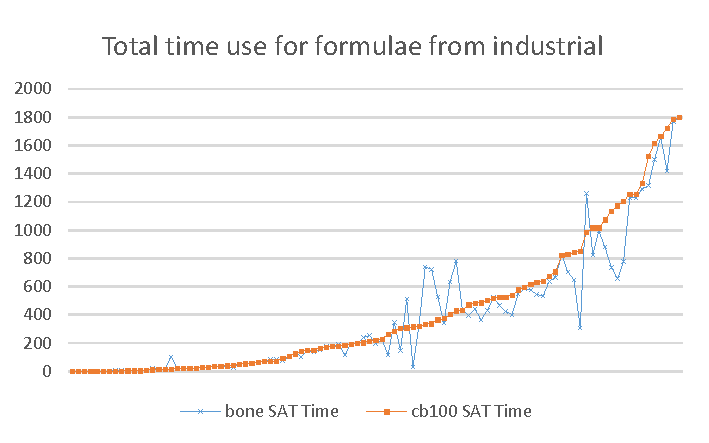
\includegraphics[scale=0.7]{ind2.pdf}
   \caption{Total time use for formulae from industrial}
   \label{fig:ind-time}
\end{figure}

\subsection{MSS Extraction Experimental Results}
In this section, we also study the performance of \tool and cb100 on random instances.
We propose a novel method to generate large number of random formulae, with the help of Maximal Satisfiable Subset(MSS) and compare the effectiveness of \tool and cb100 for MSS instances.

Given an unsatisfiable formula $\Phi$, a subset of clauses $\Phi'\subset\Phi$ is called an MSS iff for every clause $\phi\notin\Phi'$, $\Phi'$ is satisfiable and $\Phi'\wedge\phi$ is unsatisfiable. MSS is maximal satisfiable sub-formula extracted from an unsatisfiable formula. There exist a large number of different MSS for a given unsatisfiable formula. We use LBX tool to generate MSSes from random unsatisfiable benchmark. The MSS generated are also random and with a fixed upper bound of clauses count and variables count to a given unsatisfiable formula.

Our initial motivation is inspired by the result of industrial formulae.
We randomly choose 100 instances from five groups which are made according to the time for computing the first model. Figure \ref{fig:mcs-time} present the running time plot of MSS formulae. It seemed that there is no relation between the performance of backbone computing and the computing time of the first model.
It's because that random formulae have more complex community structures \cite{NZG2014,LJG2015SAT,LJG015}.

%It has been proved that the community structure of a formula related to the performance of CDCL solver \cite{NZG2014}.
%Our observation shows that the community structure of random formulae is also highly related to the performance of backbone computing.
Since it has been proved that the community structure of a formula is related to the performance of CDCL solvers \cite{NZG2014}.
We take the insight of these performance analysis, and use SATGraph \cite{NZW2015} tool to generate the community structure of formulae in MSS benchmark. We observe that cb100 performs better on formula with a long distance single vertex in a graph, shows in Figure \ref{fig:cb100}. While \tool performs better on formula with a group of vertexes around the center cluster with almost the same distance from the vertexes to the center cluster (an example is shown in Figure \ref{fig:bone}).

Based on the observation, we divide MSS benchmark into three groups according to the community structure of formulae. For formulae with a single vertex far away from center cluster, we put it to \emph{simple} group. For formulae with vertexes around the center cluster, we put it to \emph{hard} group. The rest are in \emph{medium} group. Table \ref{tab:mcs-graph} showed the result of MSS benchmark, simple(resp. medium, resp. hard) stands for the set of formulae in simple(resp.medium, resp. hard) group.

We observed that in simple group cb100 outperforms \tool. Because the essence of cb100 is trying to find a backbone literal by complementing models as soon as possible, which is exactly the single vertex literal.

For medium formulae, the total running time of \tool reduced 8\% comparing to cb100 and for hard formulae, the total running time cut off 40\%. In total, the running time of \tool is around 300 seconds less than of cb100. Based on the statistic, \tool is better than cb100 on random formulae, especially for hard random formulae.

\begin{figure}
    \centering
    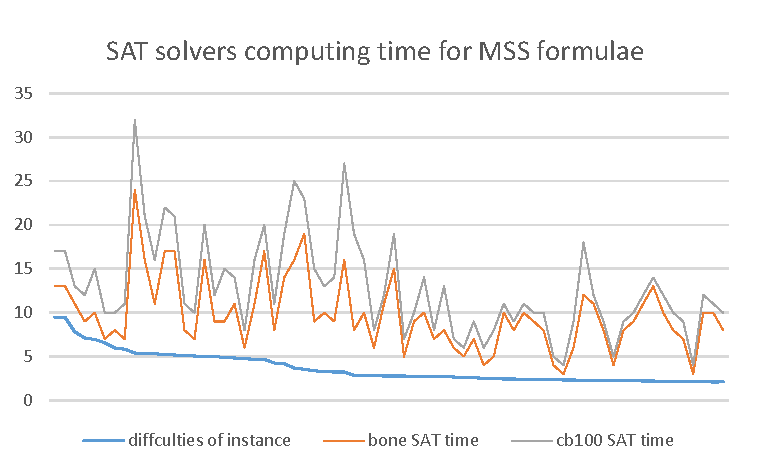
\includegraphics[scale=0.7]{mcs.pdf}
   \caption{Total time use for formulae from MCS computing}
   \label{fig:mcs-time}
\end{figure}

%\begin{figure}
%    \centering
%    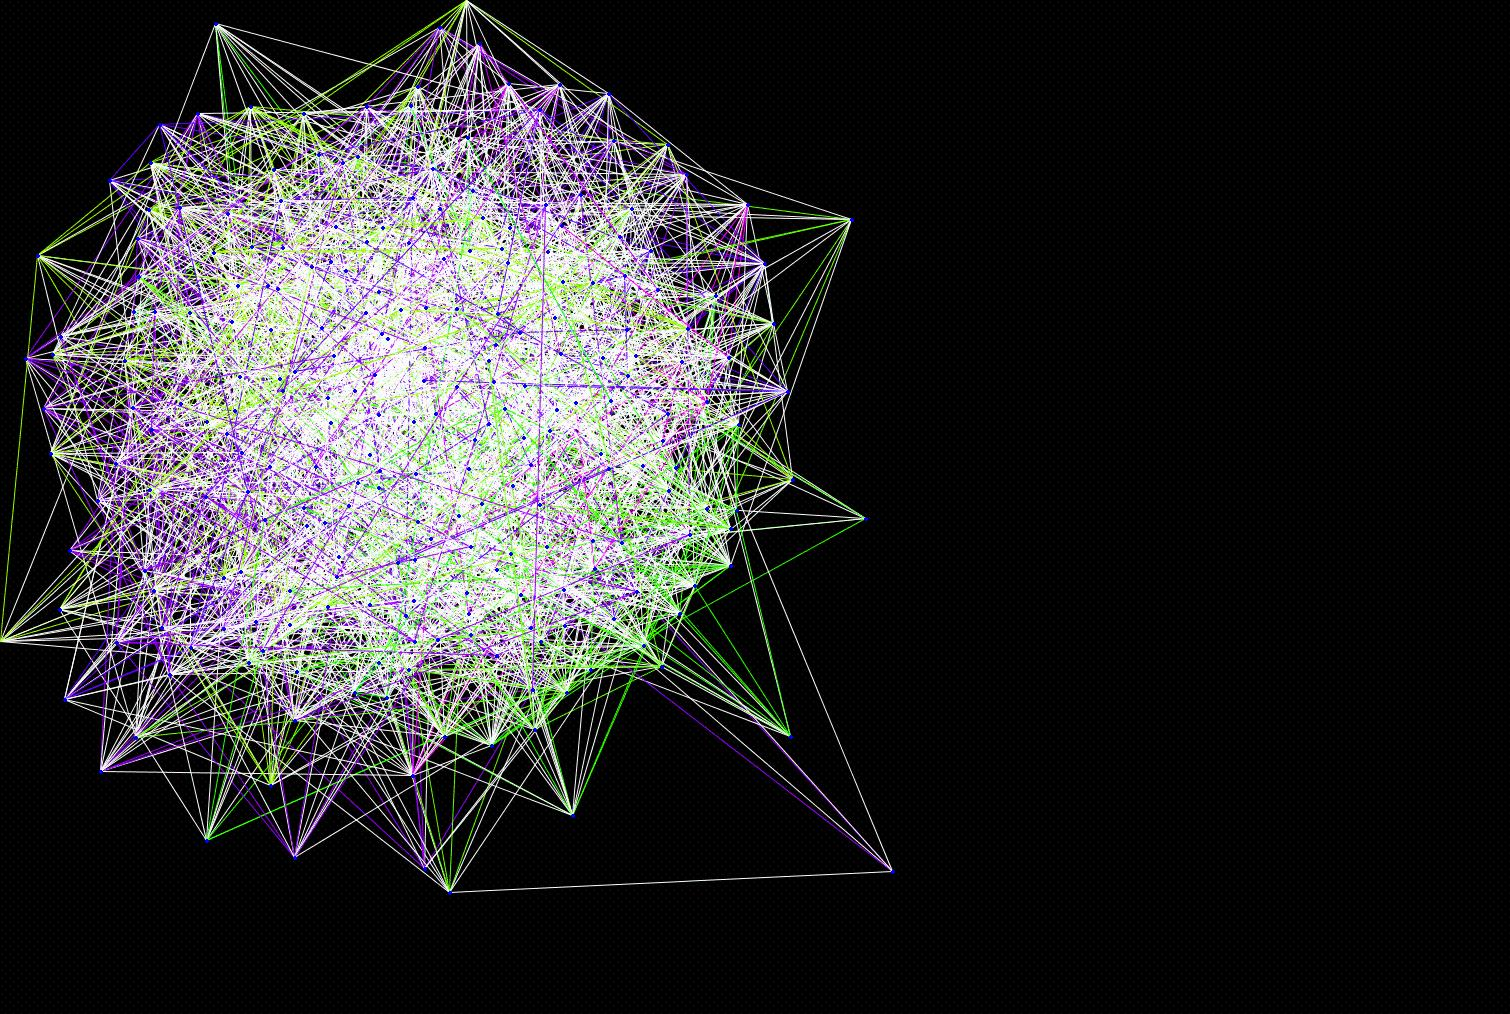
\includegraphics[scale=0.2]{cb100.jpg}
%   \caption{Community Structure of Formula Performs better with cb100}
%   \label{fig:cb100}
%\end{figure}

%\begin{figure}
%    \centering
%    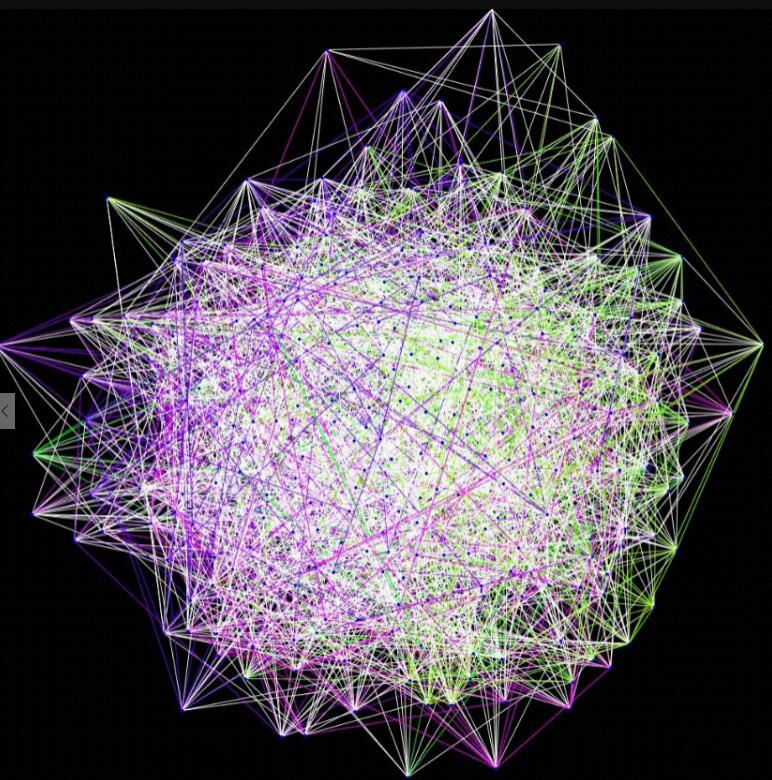
\includegraphics[scale=0.2]{bone.jpg}
%   \caption{Community Structure of Formula Performs better with \tool}
%   \label{fig:bone}
%\end{figure}

\begin{figure}[htbp]
\centering
\subfloat[cb100 performs better]{
\label{fig:cb100}
\centering
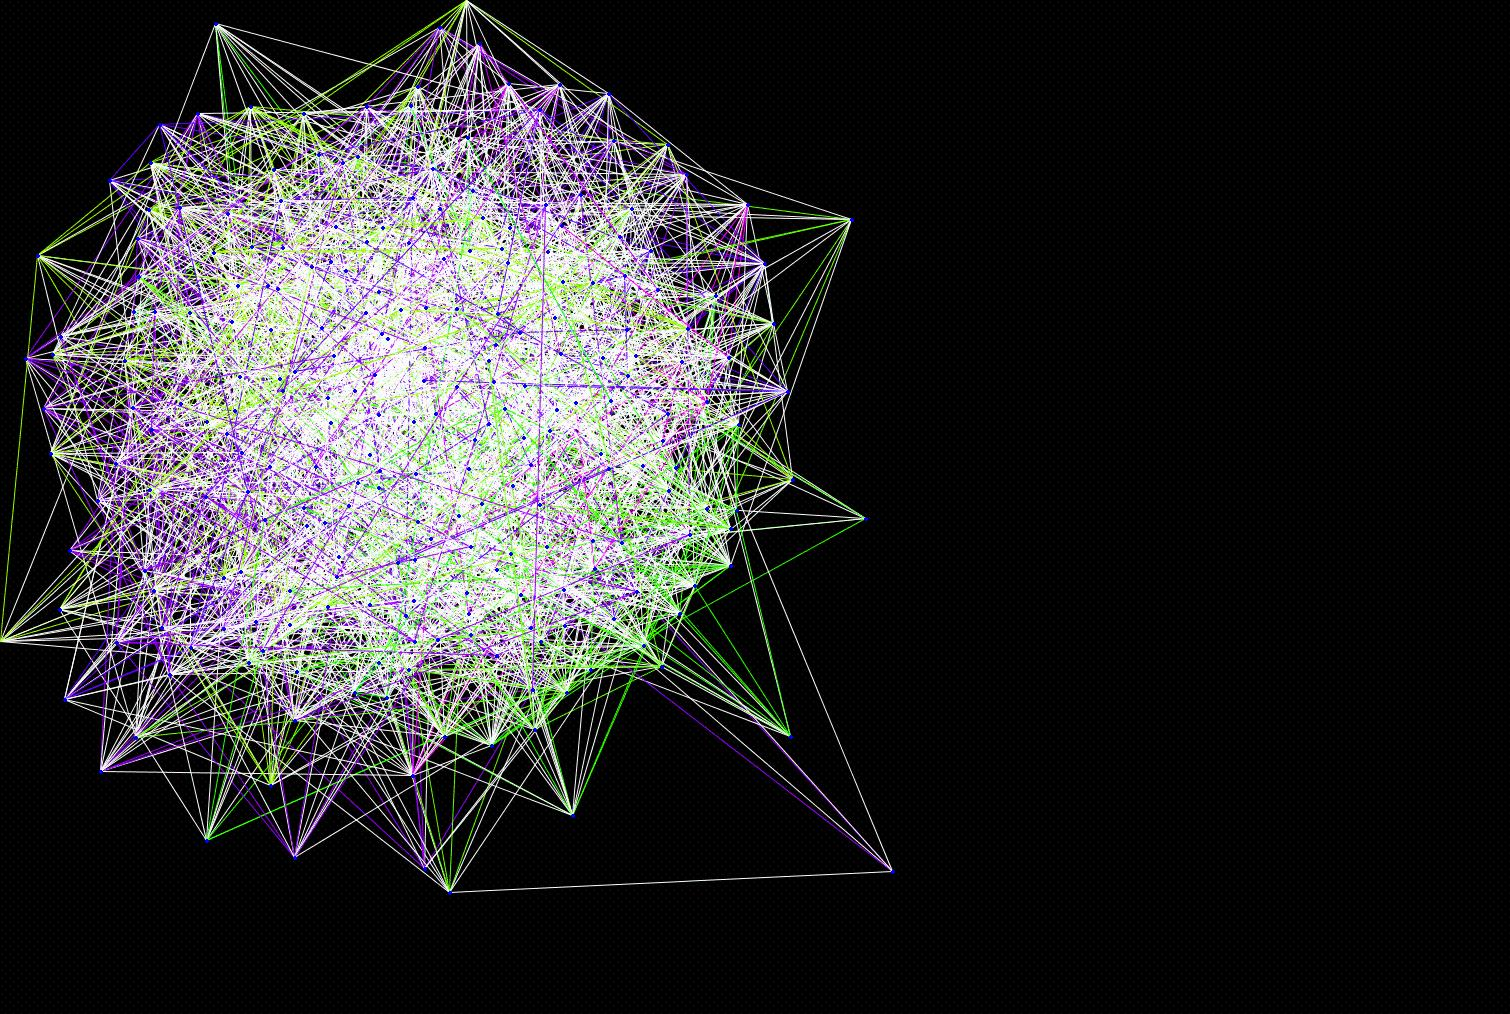
\includegraphics[width=.5\linewidth-0.45mm]{cb100.jpg}
}
\subfloat[\tool performs better]{
\label{fig:bone}
\centering
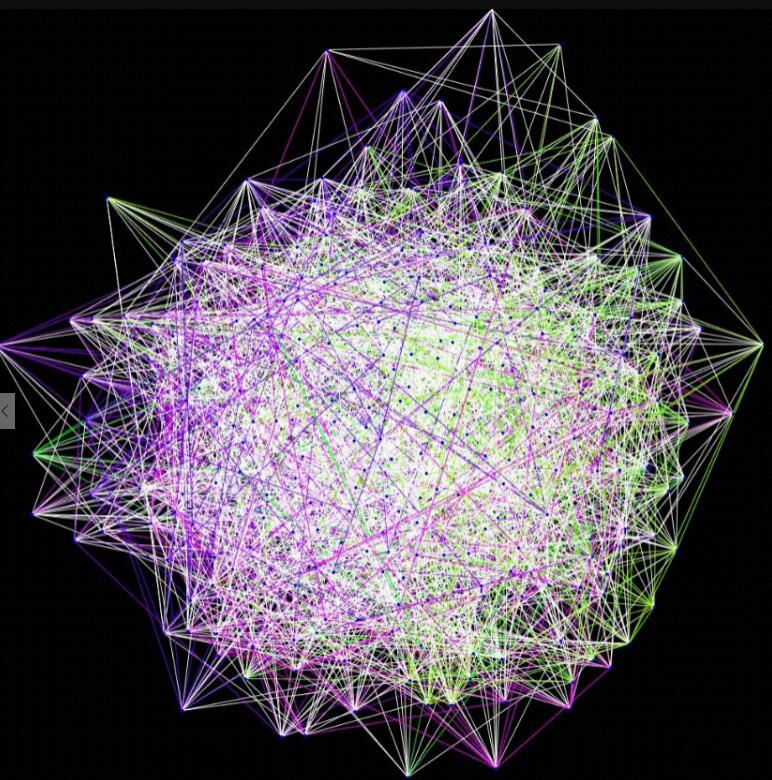
\includegraphics[width=.5\linewidth-0.45mm]{bone.jpg}
}
\caption{Community Structures of Formulae}
\end{figure}

\begin{table*}[tb]
\caption{Results of Random Formulae}
\begin{center}
\begin{tabular}{c|c|c|c|c|c|c|c|c}
\hline \hline
\multirow{2}{*}{} & \multicolumn{2}{c|}{Total}& \multicolumn{2}{c|}{Simple} & \multicolumn{2}{c|}{Medium} & \multicolumn{2}{c}{Hard} \\
\cline{2-9}
 &SAT Time & SAT Count & SAT Time & SAT Count & SAT Time & SAT Count & SAT Time & SAT Count \\
\hline
\tool & 50183.02 sec & 1508723 & 6874.5 sec & 85570 & 35853 sec & 1332334 & 3577.9 sec & 76449 \\ \hline
cb100 & 50414.04 sec & 1532372 & 4413.5 sec & 86232 & 39040 sec & 1353258 & 5893.4 sec & 78114 \\
\hline \hline
\end{tabular}
\label{tab:mcs-graph}
\end{center}
\end{table*}

From the experiments result for industrial and MSS benchmarks, we show that \tool is more efficient than cb100 on industrial formulae which need more than 120 seconds to compute the first model. We ran a benchmark of 6606 instances on random formulae and concludes that for hard group formulae, \tool has competitive advantage.





